\documentclass{beamer}
\usepackage{graphicx}
\usepackage{xcolor}
\usepackage{tikz}

\usepackage{colortbl}     % 支持 \rowcolor
\usepackage[table]{xcolor}  % 增强颜色支持，特别是灰色背景
\usepackage{array}        % 增强表格功能（对齐方式等）
\usepackage{booktabs



% 自定义颜色
\definecolor{purpleblue}{RGB}{80, 80, 180}
\definecolor{lightgray}{RGB}{230, 230, 230}
\definecolor{novelPurple}{RGB}{98, 54, 255} 
\definecolor{darkgray}{RGB}{50, 50, 50}

% 主题设置
\usetheme{Madrid}  
\usecolortheme{dolphin} 

% 设置字体（移除 fontspec，确保 pdfLaTeX 兼容）
\setbeamerfont{title}{size=\Large,series=\bfseries}
\setbeamerfont{frametitle}{size=\LARGE,series=\bfseries}
\setbeamercolor{frametitle}{fg=white, bg=novelPurple}
\setbeamercolor{title}{fg=white, bg=purpleblue}

% 封面信息
\title[Geometry Chapter 10 ]{\textbf{Geometry Chapter 10\\ Circle }}
\author{\textbf{Jack Zeng}}
\institute{\textcolor{white}{\textbf{Novel Prep}}}
\date{\today} 

\begin{document}

% --- Title Slide ---
\begin{frame}
    \titlepage
    \vfill
    \begin{flushright}
        \textcolor{purpleblue}{\Huge \textbf{Novel Prep}}
    \end{flushright}
\end{frame}




\begin{frame}
    \begin{tikzpicture}[remember picture, overlay]
        % 设置浅色渐变背景
        \shade[top color=softPurple, bottom color=softGray] 
            (current page.north west) rectangle (current page.south east);
        
        % 添加高斯模糊光晕
        \fill[white, opacity=0.3] (current page.center) circle (4cm);
        
        % 主标题
        \node[align=center] at (current page.center) {
            {\Huge\bfseries\textcolor{purpleblue}{Novel Prep}} \\[0.5cm]
            {\Large\itshape\textcolor{lightText}{Excellence in SAT Prep}}
        };

        % 添加柔和光点（点缀）
        \foreach \x in {1,2,3,4,5} {
            \fill[purpleblue, opacity=0.2] (rand*10-5, rand*7-3.5) circle (0.1+\x*0.05);
        }

        ;
    \end{tikzpicture}
\end{frame}


\begin{frame}{Overview}
    \tableofcontents
\end{frame}



\begin{frame}
\section{Radian Measure}
    \begin{tikzpicture}[remember picture, overlay]
        % 设置浅色渐变背景
        \shade[top color=softPurple, bottom color=softGray] 
            (current page.north west) rectangle (current page.south east);
        
        % 添加高斯模糊光晕
        \fill[white, opacity=0.3] (current page.center) circle (4cm);
        
        % 主标题
        \node[align=center] at (current page.center) {
            {\LARGE\bfseries\textcolor{purpleblue}{Radian Measure}} \\[0.5cm]
            {\Large\itshape\textcolor{lightText}{Excellence in SAT Prep}}
        };

        % 添加柔和光点（点缀）
        \foreach \x in {1,2,3,4,5} {
            \fill[purpleblue, opacity=0.2] (rand*10-5, rand*7-3.5) circle (0.1+\x*0.05);
        }

        ;
    \end{tikzpicture}
\end{frame}

\begin{frame}{Circle Vocabulary and Arc Measures}
\footnotesize

\textbf{Definition of a Circle:}  
A \textbf{circle} is the set of all points equidistant from a given point called the \textbf{center}. All radii are equal in measure.

\vspace{0.2cm}
\textbf{Important Terms:}
\begin{itemize}
    \item \textbf{Chord:} A segment whose endpoints lie on the circle.
    \item \textbf{Secant:} A line that intersects the circle at two points.
    \item \textbf{Tangent:} A line that touches the circle at exactly one point — the point of tangency.
    \item \textbf{Central Angle:} An angle whose vertex is at the center of the circle.
    \item \textbf{Arc:} A portion of the circle. 
\end{itemize}





\begin{center}
    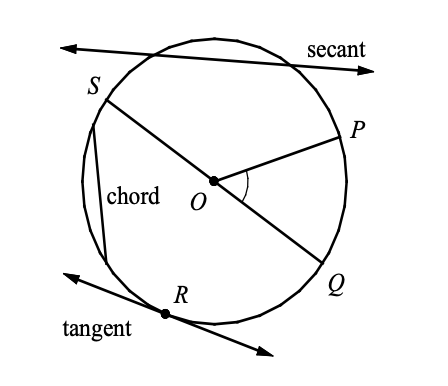
\includegraphics[width=0.4\linewidth]{E57.png}
\end{center}

\end{frame}



\begin{frame}{Understanding Radian Measure}
\small

\textbf{Definition of Radian:}  
A radian is the angle created when the arc length equals the radius.

\[
1 \text{ radian} = \frac{s}{r}
\]

\begin{itemize}
    \item $s$: Arc length
    \item $r$: Radius
\end{itemize}

\vspace{0.3cm}
\textbf{Important Note:}  
There are $2\pi$ radians in a full circle, since the circumference is $2\pi r$ and the radius is $r$.

\vspace{0.3cm}
\textbf{Degree to Radian Conversion:}
\[
\theta\ (\text{in radians}) = \theta^\circ \cdot \frac{\pi}{180}
\]

\textbf{SAT Tip:}  
Always check whether angle is given in degrees or radians before using formulas!

\end{frame}



\begin{frame}{Question: Geometry Problem Setup}
\small
In the figure below, $\overline{BD}$ is a diameter, and $\overline{PA}$ and $\overline{PD}$ are tangents to circle $O$.

\begin{itemize}
    \item $m\angle CDE = 52^\circ$
    \item $m\angle APD = 45^\circ$
    \item $AP = 9$
\end{itemize}

\begin{center}
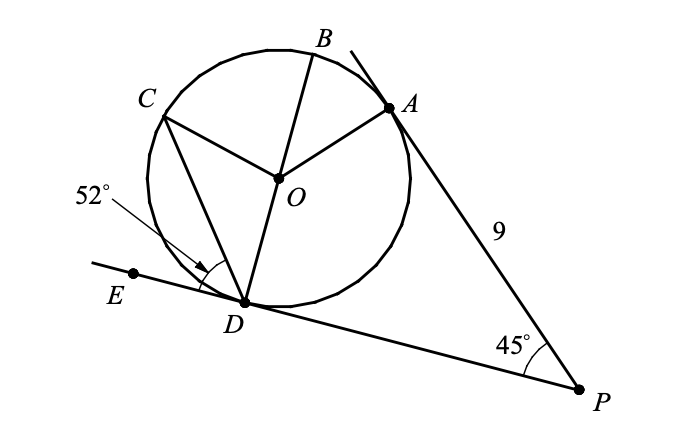
\includegraphics[width=0.4\linewidth]{E58.png}
\end{center}

\begin{itemize}


    \item {Question 1}
What is the measure of $\angle ODC$?


    \item {Question 2}
What is the measure of $\angle OCD$?

    \item {Question 3}
What is the measur of $\angle AOD$?


    \item {Question 4}
What is the length of $\overline{PD}$?
\end{itemize}
\end{frame}


\begin{frame}{Answers to Circle Geometry Questions}
\begin{enumerate}
    \item The measure of $\angle ODC$ is $90^\circ-52^\circ$. \\


    \item The measure of $\angle OCD$ is $38^\circ$. \\
    \textit{(From triangle $\triangle OCD$, we subtract $90^\circ$ and $52^\circ$ from $180^\circ$.)}

    \item The measure of $\angle AOD$ is $135^\circ$. \\


    \item The length of $\overline{PD}$ is $9$. \\
    \textit{(Using right triangle $\triangle APD$ with $\angle APD = 45^\circ$, we know it is an isosceles right triangle, so $PD = AP = 9$.)}
\end{enumerate}
\end{frame}




\section{Arc Length and Area of a Sector}
    \begin{tikzpicture}[remember picture, overlay]
        % 设置浅色渐变背景
        \shade[top color=softPurple, bottom color=softGray] 
            (current page.north west) rectangle (current page.south east);
        
        % 添加高斯模糊光晕
        \fill[white, opacity=0.3] (current page.center) circle (4cm);
        
        % 主标题
        \node[align=center] at (current page.center) {
            {\LARGE\bfseries\textcolor{purpleblue}{Arc Length and Area of a Sector}} \\[0.5cm]
            {\Large\itshape\textcolor{lightText}{Excellence in SAT Prep}}
        };

        % 添加柔和光点（点缀）
        \foreach \x in {1,2,3,4,5} {
            \fill[purpleblue, opacity=0.2] (rand*10-5, rand*7-3.5) circle (0.1+\x*0.05);
        }

        ;
    \end{tikzpicture}
\end{frame}


\begin{frame}{Arc Length of a Circle}
\small

\textbf{Arc Length Formula:}
\[
s = r\theta
\]
\textit{(where $s$ = arc length, $r$ = radius, $\theta$ = central angle in radians)}

\vspace{0.3cm}
\textbf{Example:}  
Find the arc length of a circle with:
\begin{itemize}
    \item Radius: $r = 6$
    \item Central angle: $\theta = 60^\circ = \frac{\pi}{3}$ radians
\end{itemize}

\vspace{0.2cm}
\[
s = r\theta = 6 \cdot \frac{\pi}{3} = 2\pi
\]

\vspace{0.3cm}
\textbf{SAT Tip:}  
Do not use this formula unless $\theta$ is in radians!

\end{frame}





\begin{frame}{Area of a Sector}
\small

\textbf{Definition:}  
A sector is a "pizza slice" portion of a circle.

\textbf{Formula (Radians):}
\[
\text{Area} = \frac{1}{2} r^2 \theta
\]

\vspace{0.3cm}
\textbf{Formula (Degrees):}
\[
\text{Area} = \frac{\theta^\circ}{360^\circ} \cdot \pi r^2
\]

\vspace{0.3cm}
\textbf{Example:}  
Find the area of a sector of a circle with radius 4 and angle $45^\circ$:

\[
\text{Area} = \frac{45}{360} \cdot \pi \cdot 4^2 = \frac{1}{8} \cdot 16\pi = 2\pi
\]

\vspace{0.2cm}
\textbf{SAT Reminder:} Be sure whether angle is in radians or degrees before using a formula.

\end{frame}


\begin{frame}{\textbf{Question: Arc Length and Central Angle}}

\begin{center}
    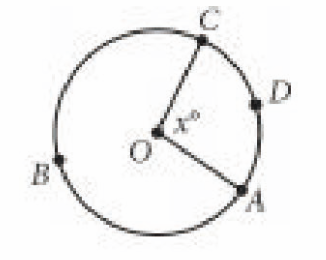
\includegraphics[width = 0.3\linewidth]{E39.png}
\end{center}

The circle above has center \( O \), the length of arc \( \widehat{ADC} \) is \( 5\pi \), and \( x = 100 \).  
What is the length of arc \( \widehat{ABC} \)?

\begin{itemize}
    \item[A.] \( 9\pi \)
    \item[B.] \( 13\pi \)
    \item[C.] \( 18\pi \)
    \item[D.] \( \frac{13}{2}\pi \)
\end{itemize}
\end{frame}


\begin{frame}{\textbf{Answer: Arc Length and Central Angle}}
We are told:
\begin{itemize}
    \item \( \text{Length of arc } \widehat{ADC} = 5\pi \)
    \item Central angle \( \angle AOC = x = 100^\circ \)
\end{itemize}

Since the entire circle represents \( 360^\circ \), the arc \( \widehat{ABC} \) must span:
\[
360^\circ - 100^\circ = 260^\circ
\]

Using the proportion of arc to full circle:
\[
\frac{260}{100} = \frac{\text{Length of } \widehat{ABC}}{\text{Length of } \widehat{ADC}} = \frac{L}{5\pi}
\Rightarrow L = 5\pi \cdot \frac{260}{100} = 13\pi
\]

\textbf{Correct Answer:} \fbox{\( \text{B. } 13\pi \)}
\end{frame}



\begin{frame}
\section{Properties of the Circle}
    \begin{tikzpicture}[remember picture, overlay]
        % 设置浅色渐变背景
        \shade[top color=softPurple, bottom color=softGray] 
            (current page.north west) rectangle (current page.south east);
        
        % 添加高斯模糊光晕
        \fill[white, opacity=0.3] (current page.center) circle (4cm);
        
        % 主标题
        \node[align=center] at (current page.center) {
            {\LARGE\bfseries\textcolor{purpleblue}{Properties of the Circle}} \\[0.5cm]
            {\Large\itshape\textcolor{lightText}{Excellence in SAT Prep}}
        };

        % 添加柔和光点（点缀）
        \foreach \x in {1,2,3,4,5} {
            \fill[purpleblue, opacity=0.2] (rand*10-5, rand*7-3.5) circle (0.1+\x*0.05);
        }

        ;
    \end{tikzpicture}
\end{frame}

\begin{frame}{Angles Inscribed in a Semicircle}
\small

\textbf{Theorem:}  
Any angle inscribed in a semicircle is a \textbf{right angle (90°)}.

\begin{itemize}
    \item If a triangle is inscribed in a circle and one side is the diameter, then the angle opposite that side is $90^\circ$.
\end{itemize}

\vspace{0.2cm}
\textbf{Example:}  
If triangle $ACB$ is inscribed in a circle and $AB$ is a diameter, then:
\[
\angle C = 90^\circ
\]

\begin{center}
    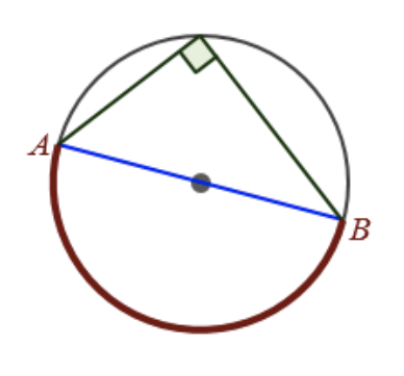
\includegraphics[width=0.3\linewidth]{E35.png}
\end{center}

\textbf{SAT Tip:}  
Look for a triangle with one side as a diameter — it’s a right triangle!

\end{frame}

\begin{frame}{Radius and Tangent Line}
\small

\textbf{Key Property:}  
The radius of a circle is \textbf{perpendicular} to the tangent line at the point of contact.

\begin{center}
    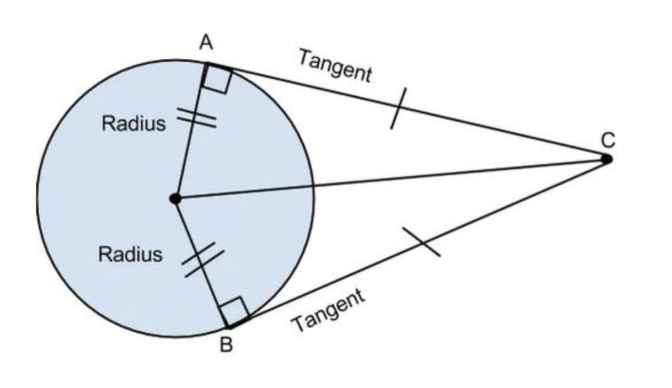
\includegraphics[width=0.4\linewidth]{E36.png}
\end{center}

\begin{itemize}
    \item Use this right angle in triangle questions.
    \item Often used in slope problems — if radius has slope $m$, tangent has slope $-\frac{1}{m}$.
\end{itemize}


\textbf{SAT Tip:}  
If the question mentions “tangent”, check for perpendicularity with radius.

\end{frame}







\begin{frame}{Inscribed Angles and Their Properties}
\small

\textbf{Inscribed Angle:}  
An \textbf{inscribed angle} is formed by two chords in a circle that share an endpoint. The vertex lies on the circle.

\vspace{0.2cm}
\textbf{Inscribed Angle Theorem:}  
The measure of an inscribed angle is half the measure of its intercepted arc:
\[
m\angle B = \frac{1}{2}m\overset{\frown}{AC} = \frac{1}{2}m\angle AOC
\]

\vspace{0.2cm}
\begin{center}
    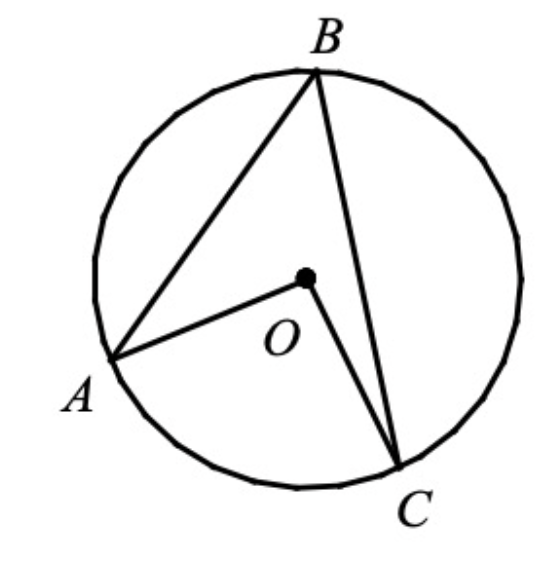
\includegraphics[width=0.4\linewidth]{E59.png}
\end{center}

\end{frame}


\begin{frame}{Congruent Inscribed Angles}
\small

\textbf{Key Concept:}  
\textbf{Inscribed angles} that intercept the same arc are \textbf{congruent}.

\vspace{0.2cm}
This means:
\[
\angle A \cong \angle B
\quad \text{if they intercept the same arc.}
\]

\vspace{0.2cm}
\begin{center}
    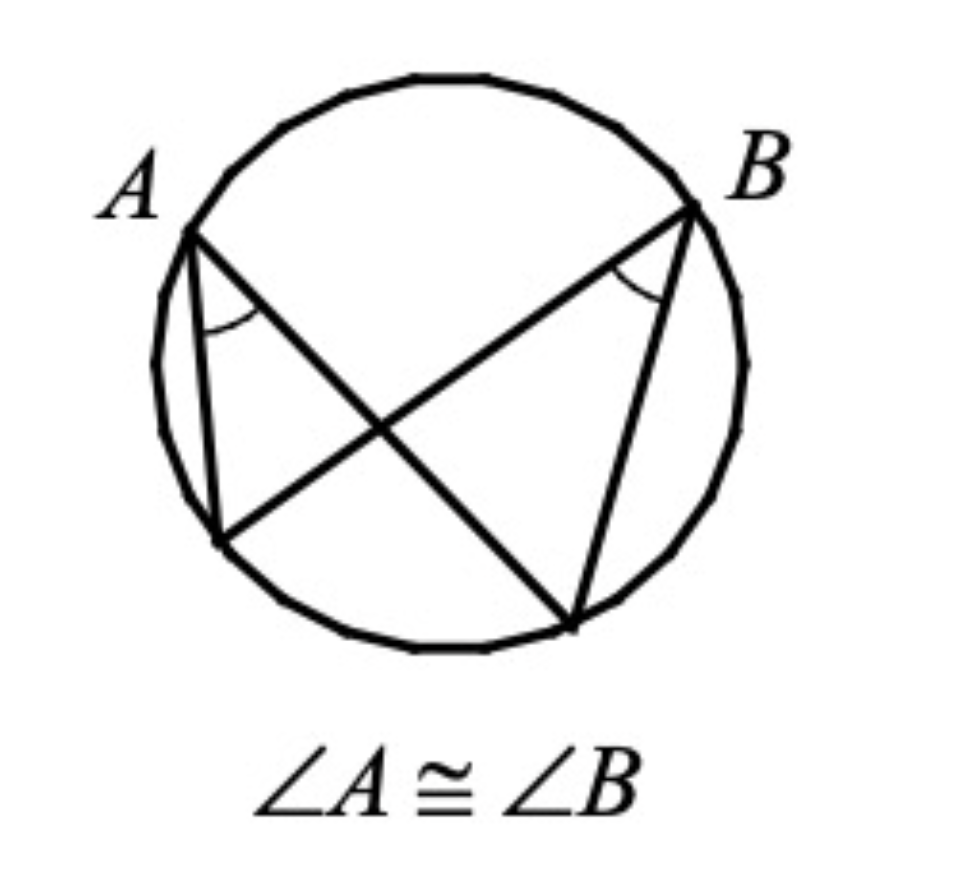
\includegraphics[width=0.4\linewidth]{E60.png}
\end{center}

\end{frame}



\begin{frame}{Cyclic Quadrilaterals}
\small

\textbf{Cyclic Quadrilateral:}  
A quadrilateral inscribed in a circle.

\vspace{0.2cm}
\textbf{Property:}  
Opposite angles of a cyclic quadrilateral are \textbf{supplementary}.
\[
\angle A + \angle C = 180^\circ,\quad \angle B + \angle D = 180^\circ
\]

\vspace{0.2cm}
\begin{center}
    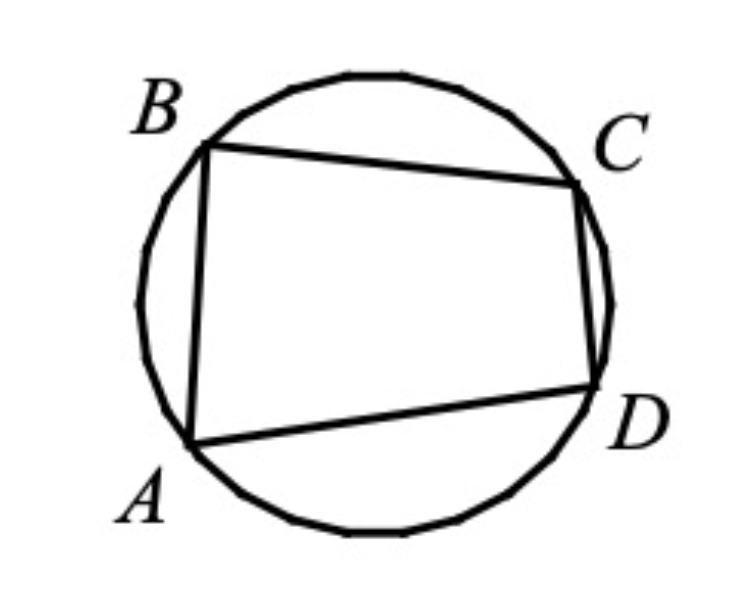
\includegraphics[width=0.4\linewidth]{E61.png}
\end{center}

\end{frame}





\begin{frame}{Radius Bisecting a Chord}
\small

\textbf{Theorem:}  
If a radius (or diameter) is perpendicular to a chord, it \textbf{bisects} the chord.

\vspace{0.2cm}
\[
\text{If } AB \perp OE,\ \text{then } AD = DB
\]

\begin{center}
    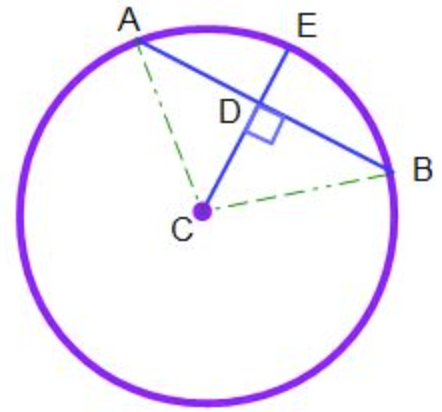
\includegraphics[width=0.20\linewidth]{E37.png}
\end{center}


\begin{itemize}
    \item Can be used to find missing lengths using right triangle properties.
    \item Also useful for coordinate geometry questions involving symmetry.
\end{itemize}

\textbf{Note:} The converse is also true — if a radius bisects a chord, it’s perpendicular.

\vspace{0.3cm}
\textbf{Useful for:} Midpoint formula, Pythagorean theorem, and algebraic proofs.

\end{frame}

\begin{frame}{Congruent Arcs and Chords}
\small

\textbf{Theorem:}  
In the same circle or in congruent circles, congruent arcs have congruent chords.  
The converse is also true.

\[
\text{If } \widehat{AB} \cong \widehat{CD}, \text{ then } \overline{AB} \cong \overline{CD}
\]

\vspace{0.3cm}
\begin{center}
    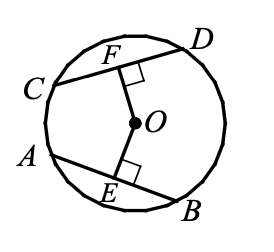
\includegraphics[width=0.45\linewidth]{E63}
\end{center}

\end{frame}


\begin{frame}{Congruent Arcs and Chords}
\small

\textbf{Theorem:}  
In the same circle or in congruent circles, congruent arcs have congruent chords.  
The converse is also true.

\[
\text{If } \widehat{AB} \cong \widehat{CD}, \text{ then } \overline{AB} \cong \overline{CD}
\]

\vspace{0.3cm}
\begin{center}
    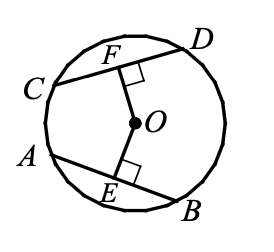
\includegraphics[width=0.45\linewidth]{E63}
\end{center}

\end{frame}



\begin{frame}{\textbf{Question: Arc Length in Circle Geometry}}

\begin{center}
    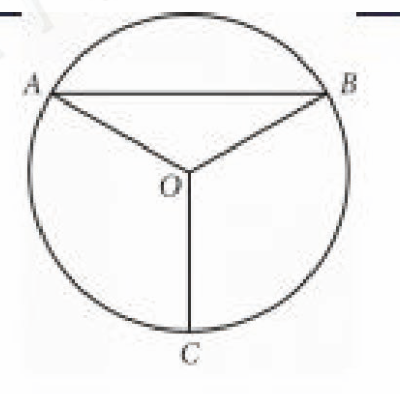
\includegraphics[width=0.3\linewidth]{E38.png}
\end{center}
Point \( O \) is the center of the circle above, and the measure of \( \angle OAB \) is \( 30^\circ \).  
If the length of \( \overline{OC} \) is \( 18 \), what is the length of arc \( \widehat{AB} \)?

\begin{itemize}
    \item[A.] \( 9\pi \)
    \item[B.] \( 12\pi \)
    \item[C.] \( 15\pi \)
    \item[D.] \( 18\pi \)
\end{itemize}
\end{frame}




\begin{frame}{\textbf{Answer: Arc Length in Circle Geometry}}
Since \( \angle OAB = 30^\circ \), the central angle for arc \( AB \) is \( 60^\circ \) (as it spans angle \( AOB \)).  
The radius is \( r = 18 \), so the circumference of the full circle is:
\[
C = 2\pi r = 2\pi(18) = 36\pi.
\]
The arc \( \widehat{AB} \) represents \( \frac{120^\circ}{360^\circ} = \frac{1}{3} \) of the full circle, so its length is:
\[
\frac{1}{3} \times 36\pi = 12\pi.
\]

\textbf{Correct Answer:} \fbox{\( 12\pi \)}  

\end{frame}



\begin{frame}{Chord-Chord Power Theorem}
\small
\textbf{Theorem:} If two chords intersect in a circle, then the products of the lengths of the chord segments are equal.

\[
HA \cdot AJ = IA \cdot AK
\]

\vspace{0.3cm}
\textbf{Key Concept:}  
This relationship holds when two chords intersect inside the circle, forming two segments on each chord.

\begin{center}
    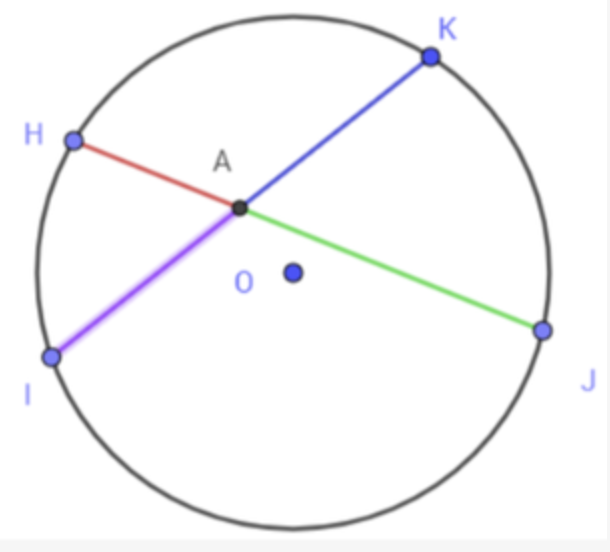
\includegraphics[width=0.4\linewidth]{E51.png}
\end{center}

\end{frame}


\begin{frame}{Secant-Secant Power Theorem}
\small
\textbf{Theorem:} If two secants intersect in the exterior of a circle, then the product of the measures of one secant and its external segment equals the same product for the other.

\[
PM \cdot PL = PO \cdot PN
\]

\vspace{0.3cm}
\textbf{Key Insight:}  
The external part times the whole secant length gives a consistent value across both secants.

\begin{center}
    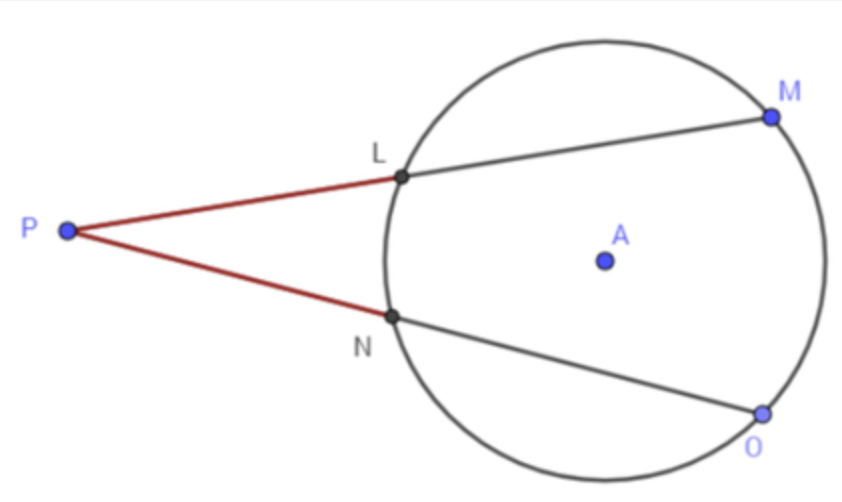
\includegraphics[width=0.4\linewidth]{E52}
\end{center}
\end{frame}


\begin{frame}{Secant-Tangent Power Theorem}
\small
\textbf{Theorem:} If a secant and a tangent intersect in the exterior of a circle, then the square of the tangent is equal to the product of the secant and its external part.

\[
PM^2 = PN \cdot PO
\]

\vspace{0.3cm}
\textbf{Key Tip:}  
This is a special case of the secant-secant relationship where one of the secants becomes a tangent (only touches the circle once).

\begin{center}
    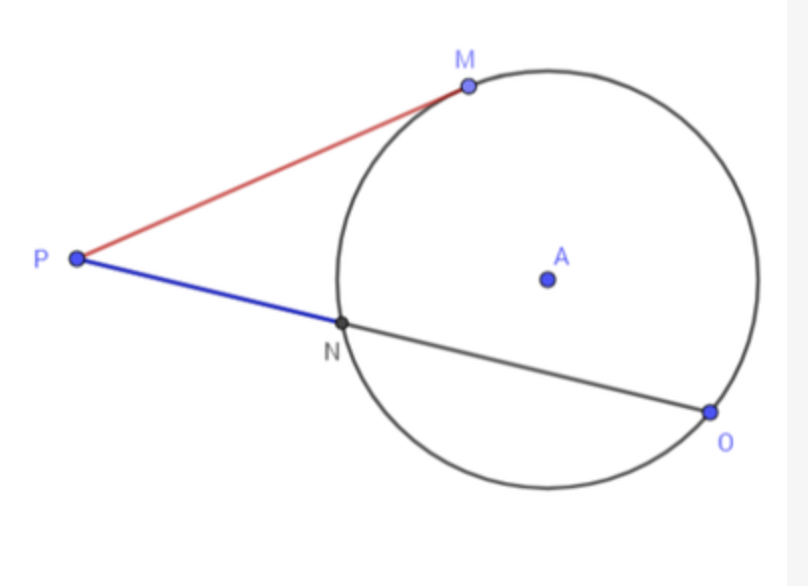
\includegraphics[width=0.4\linewidth]{E53.png}
\end{center}
\end{frame}


\begin{frame}{Question: Chord-Chord Power Theorem}
Solve for $x$.
\begin{center}
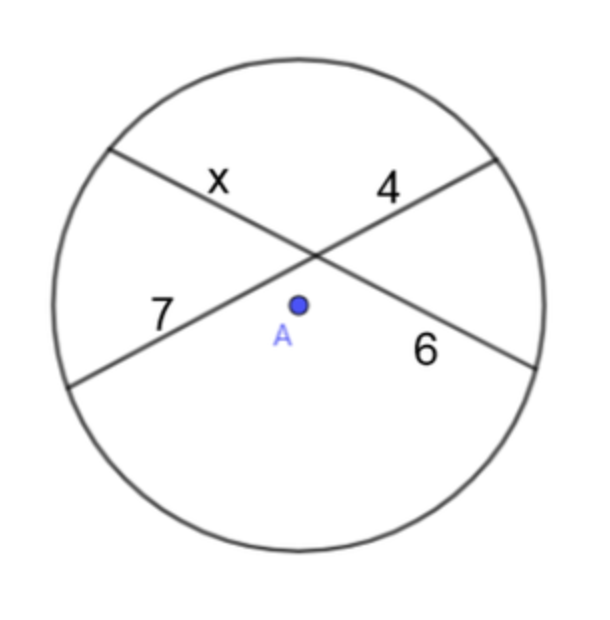
\includegraphics[width=0.4\linewidth]{E54.png}
\end{center}
\end{frame}

\begin{frame}{Solution}
Using the Chord-Chord Power Theorem:
\[
7 \cdot 4 = 6x
\]
\[
28 = 6x
\]
\[
x = \frac{14}{3}
\]
\end{frame}


\begin{frame}{Example : Secant-Secant Power Theorem}
Solve for $x$.
\begin{center}
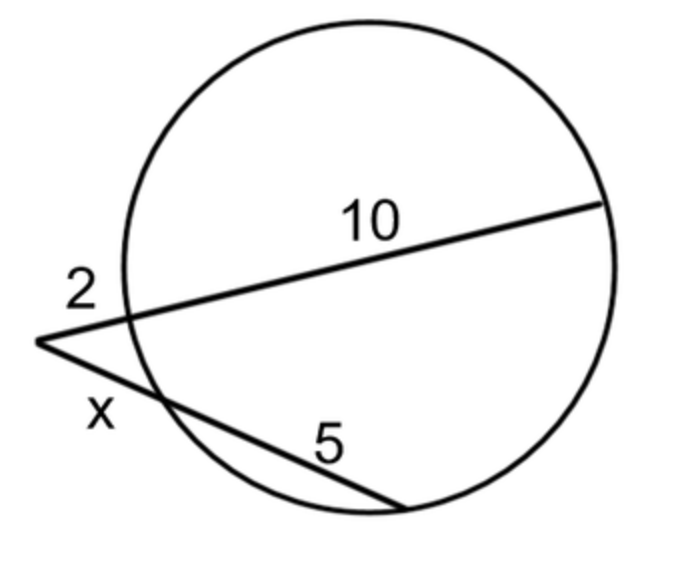
\includegraphics[width=0.4\linewidth]{E55.png}
\end{center}
\end{frame}

\begin{frame}{Solution}
Using the Secant-Secant Power Theorem:
\[
2 \cdot 12 = x(x + 5)
\]
\[
24 = x^2 + 5x
\]
\[
0 = x^2 + 5x - 24
\]
\[
0 = (x - 3)(x + 8)
\]
\[
x = 3 \quad \text{or} \quad x = -8
\]
Only $x = 3$ is a valid solution because length must be positive.
\end{frame}


\begin{frame}{Example : Secant-Tangent Power Theorem}
Given the diagram with a tangent segment, solve for $x$.
\begin{center}
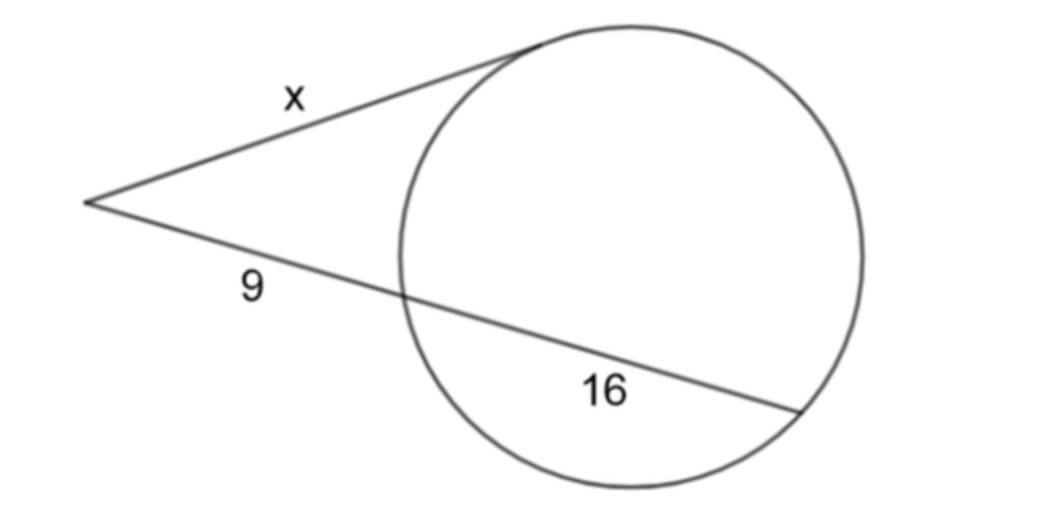
\includegraphics[width=0.6\linewidth]{E56.png}
\end{center}
\end{frame}

\begin{frame}{Solution}
Using the Secant-Tangent Power Theorem:
\[
x^2 = (9)(25)
\]
\[
x^2 = 225
\]
\[
x = \pm\sqrt{225} = \pm 15
\]
Only $x = 15$ is a valid solution because length must be positive.
\end{frame}


\begin{frame}
\section{Equation of a Circle in XY-Plane}
    \begin{tikzpicture}[remember picture, overlay]
        % 设置浅色渐变背景
        \shade[top color=softPurple, bottom color=softGray] 
            (current page.north west) rectangle (current page.south east);
        
        % 添加高斯模糊光晕
        \fill[white, opacity=0.3] (current page.center) circle (4cm);
        
        % 主标题
        \node[align=center] at (current page.center) {
            {\LARGE\bfseries\textcolor{purpleblue}{Equation of a Circle in XY-Plane}} \\[0.5cm]
            {\Large\itshape\textcolor{lightText}{Excellence in SAT Prep}}
        };

        % 添加柔和光点（点缀）
        \foreach \x in {1,2,3,4,5} {
            \fill[purpleblue, opacity=0.2] (rand*10-5, rand*7-3.5) circle (0.1+\x*0.05);
        }

        ;
    \end{tikzpicture}
\end{frame}



\begin{frame}{Equation of a Circle (Coordinate Plane)}
\small

\textbf{Standard Form:}
\[
(x - h)^2 + (y - k)^2 = r^2
\]

\textbf{Where:}
\begin{itemize}
    \item $(h, k)$ is the center,
    \item $r$ is the radius.
\end{itemize}

\vspace{0.2cm}
\textbf{Example:}  
Circle with center $(3, -2)$ and radius $5$:
\[
(x - 3)^2 + (y + 2)^2 = 25
\]

\textbf{SAT Skills:}
\begin{itemize}
    \item Completing the square to rewrite equations.
    \item Identify center and radius from expanded forms.
\end{itemize}

\end{frame}



\begin{frame}{Completing the Square to Find Circle Equation}
\small

\textbf{Given:}  
\[
x^2 + y^2 - 6x + 8y + 9 = 0
\]

\vspace{0.2cm}
\textbf{Steps:}
\begin{enumerate}
    \item Group $x$ and $y$ terms:
    \[
    (x^2 - 6x) + (y^2 + 8y) = -9
    \]
    \item Complete the square:
    \[
    (x - 3)^2 - 9 + (y + 4)^2 - 16 = -9
    \]
    \item Simplify:
    \[
    (x - 3)^2 + (y + 4)^2 = 16
    \]
\end{enumerate}

\vspace{0.2cm}
\textbf{Final Answer:} Center = $(3, -4)$, Radius = $4$

\textbf{SAT Tip:} Always isolate constants and complete square carefully on both $x$ and $y$ terms.

\end{frame}

\begin{frame}{\textbf{Question: Completing the Square }}

The graph of the equation 
\[
x^2 + x + y^2 + y = \frac{199}{2}
\]
in the \(xy\)-plane is a circle. What is the length of the circle’s radius?
\end{frame}


\begin{frame}{\textbf{Answer: Completing the Square – Radius of a Circle}}
\small
To convert the given equation to the standard form of a circle, complete the square for both \(x\) and \(y\):

\[
x^2 + x + y^2 + y = \frac{199}{2}
\]

Complete the square:

\[
x^2 + x = \left(x + \frac{1}{2}\right)^2 - \frac{1}{4}, \quad y^2 + y = \left(y + \frac{1}{2}\right)^2 - \frac{1}{4}
\]

So,

\[
\left(x + \frac{1}{2}\right)^2 - \frac{1}{4} + \left(y + \frac{1}{2}\right)^2 - \frac{1}{4} = \frac{199}{2}
\]

\[
\left(x + \frac{1}{2}\right)^2 + \left(y + \frac{1}{2}\right)^2 = \frac{199}{2} + \frac{1}{2} = \frac{200}{2} = 100
\]

Thus, the radius is:

\[
r = \sqrt{100} = 10
\]
\end{frame}

\end{document}